\documentclass[tikz,border=4pt]{standalone}
\usepackage{pgfplots}\usepgfplotslibrary{groupplots}
\pgfplotsset{compat=1.18}
\definecolor{corba}{HTML}{365FB3}\definecolor{guia}{HTML}{7C3AED}\definecolor{punt}{HTML}{B91C1C}
\begin{document}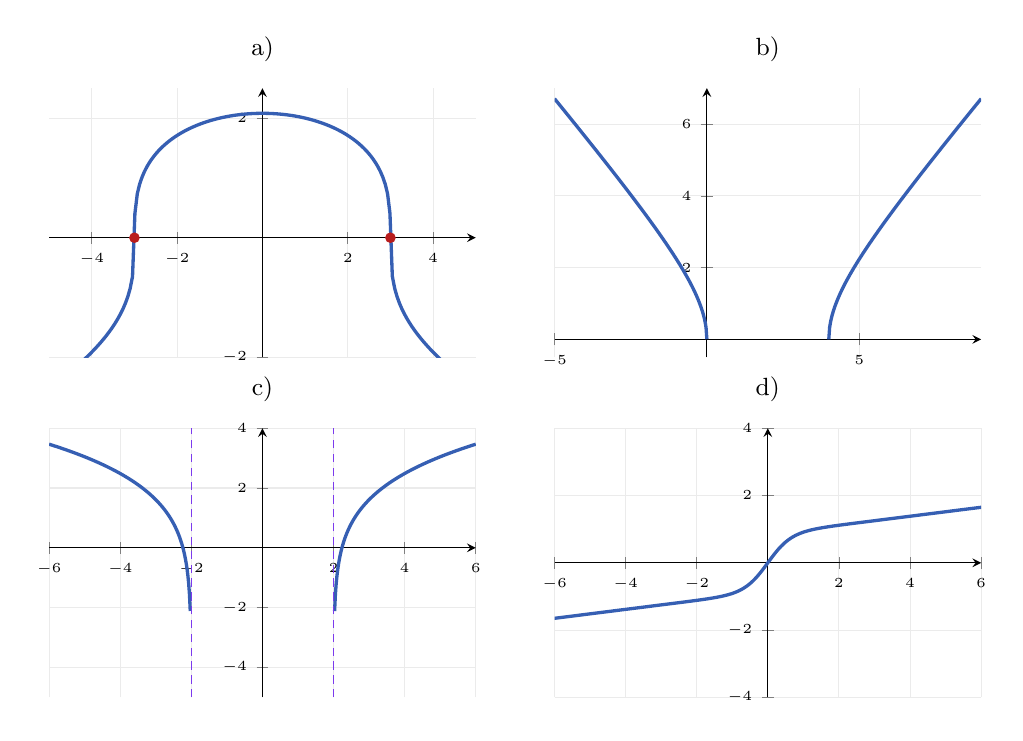
\begin{tikzpicture}
\begin{groupplot}[group style={group size=2 by 2,horizontal sep=1cm,vertical sep=0.9cm},width=7cm,height=5cm,
 axis lines=middle,grid=major,grid style={black!8},tick label style={font=\tiny},title style={font=\small},samples=180]
\nextgroupplot[title={a)},xmin=-5,xmax=5,ymin=-2,ymax=2.5]\addplot[corba,very thick,domain=-5:5]{(abs(9-x^2))^(1/3)*(9-x^2>=0 ? 1 : -1)};
 \addplot[only marks,mark=*,mark size=1.7pt,punt] coordinates {(-3,0)(3,0)};
\nextgroupplot[title={b)},xmin=-5,xmax=9,ymin=-.5,ymax=7]\addplot[corba,very thick,domain=-5:0]{sqrt(x^2-4*x)};\addplot[corba,very thick,domain=4:9]{sqrt(x^2-4*x)};
\nextgroupplot[title={c)},xmin=-6,xmax=6,ymin=-5,ymax=4]\addplot[corba,very thick,domain=-6:-2.03]{ln(x^2-4)};\addplot[corba,very thick,domain=2.03:6]{ln(x^2-4)};\addplot[guia,densely dashed] coordinates {(-2,-5)(-2,4)};\addplot[guia,densely dashed] coordinates {(2,-5)(2,4)};
\nextgroupplot[title={d)},xmin=-6,xmax=6,ymin=-4,ymax=4]\addplot[corba,very thick,domain=-6:6]{x/ln(x^2+2)};
\end{groupplot}\end{tikzpicture}\end{document}
